\documentclass[12pt,a4paper,notitlepage]{article}
% dans ce modèle article ne pas utiliser la mention "chapter", par contre on peut
% utiliser la numérotation naturelle et les références croisées.
\usepackage[utf8x]{inputenc}
%\usepackage{ucs}
\usepackage[french]{babel}
\usepackage[T1]{fontenc}
%\usepackage{eurosym} % pour pouvoir utiliser le symbole \euro{}
\usepackage[left=17mm,right=17mm,top=17mm,bottom=17mm]{geometry}
% définition du nombre de lignes à afficher en fin ou en début de page pour
% éviter les veuves et orphelines.
\usepackage[all, defaultlines=3]{nowidow}
\usepackage{array}
\usepackage[table]{xcolor} % pour couleur de blocs, permis avec \color{couleur}{texte}

\usepackage{multirow}
\usepackage{multicol}
	\setlength{\columnsep}{0.6cm}
	\setlength{\columnseprule}{1pt}
	\def\columnseprulecolor{\color{black}}

%\usepackage{wrapfig}
% \begin{wrapfigure}[lineheight]{position = r R l L i I o O}{width}
%  minuscule = float, majuscule = force emplacement
% \end{wrapfigure}

\usepackage{hyperref} %support des url via le tag \url
\hypersetup{
	colorlinks=true,
	linkcolor=blue,
	urlcolor=purple,
	}
	\urlstyle{same}
\usepackage{amsmath}
\usepackage{amsfonts}
\usepackage{amssymb}
	\everymath{\displaystyle}
%\usepackage{textcomp}

\usepackage{graphicx}
%\graphicspath{ {./Images/} } % indique le chemin relatif où sont situées les images
% définition de la clé Graphic Inclusion pour paramétrer par défaut la taille des images incluses
	\setkeys{Gin}{width=0.5000\linewidth}
\usepackage{float}
	\floatplacement{table}{H} %par défaut tables là où code est posé
	\floatplacement{figure}{H} %par défaut images là où code est posé
\usepackage{siunitx}
	\sisetup{locale = FR}
%%%% Packet circuitikz permet de dessiner des circuits électriques, peut nécessiter l'utiliation de siunitx
%\usepackage[european]{circuitikz}
%\usetikzlibrary{babel}
%\usepackage{qrcode}
%\usepackage{pgfplots} %permet de tracer directement des graphiques depuis latex

\usepackage{ifthen}
%%% Gestion de la dyslexie
\newboolean{isDyslexique}
	\setboolean{isDyslexique}{False}
%%% Gestion de la correction
\newboolean{isCorrection}
	\setboolean{isCorrection}{False}
\newboolean{isEvaluation}
	\setboolean{isEvaluation}{False}

% \usepackage{palatino} %\usepackage{sans}
% \usepackage{lxfonts} %\usepackage{arev}
\ifthenelse{\boolean{isDyslexique}}{% si vrai :
	\usepackage{arev}
	\renewcommand{\baselinestretch}{1.5}
}{% si faux :
	\usepackage{lmodern}
	\renewcommand{\baselinestretch}{1.25}
}
\usepackage{lastpage}
% test de modification des headers et footers
\usepackage{fancyhdr}
\pagestyle{fancy}
\fancyhf{}
\fancyhead[LE,RO]{\rightmark}
\fancyhead[LO,RE]{\leftmark}
\fancyfoot[LE,RO]{F.S.G.}
\fancyfoot[C]{.::--- \ \thepage / \pageref*{LastPage} \ ---::.}
\fancyfoot[RE,LO]{c4-3.pd.acxx}
% fin du test de modification :)
\usepackage{tikz}
	\usetikzlibrary{babel,math}
% inclusion du paquet bclogo pour boîtes avec logo de mise en exergue
\usepackage[tikz]{bclogo}

% ========= DÉFINITION D'UN INTERLIGNE DIFFÉRENT ===============
\setlength{\parskip}{0.1cm} % définit l'espacement entre paragraphes
\renewcommand{\thesection}{\Roman{section}}

\author{F.G.}
% éviter le titre peut-être ?
\title{}

\begin{document}

\begin{flushleft}
\begin{tabular}{| m{0.15\linewidth}  m{0.8\linewidth} || }
	\hline
	\multirow{4}{*}{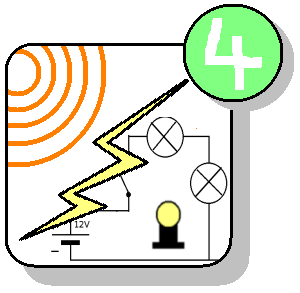
\includegraphics[width=\linewidth]{cycle4-logo-elec-ondes-nrj.png}} 
	& c4-3·pd·ac
	\begin{LARGE}
		T.P. : Description des signaux sonores.
	\end{LARGE} \cr
	\cline{2-2}
	 & \cr
	 & Nom : . \ \ . \ \ . \ \ . \ \ . \ \ . \ \ . \ \ . Prénom : . \ \ . \ \ . \ \ . \ \ . \ \ . \cr
	 & \cr
	 & Classe / Groupe : . \ \ . \ \ . \ \ . Durée : ..... min. \cr
	\hline\hline
\end{tabular}
\end{flushleft}

% ======== LISTE DES IMAGES DISPONIBLES POUR CYCLES 3 ET 4 =========
% 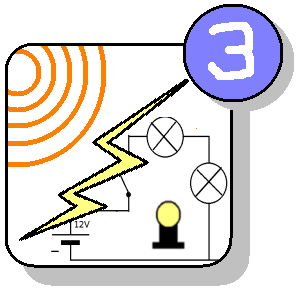
\includegraphics[scale=0.333]{cycle3-logo-elec-ondes-nrj.png}
% 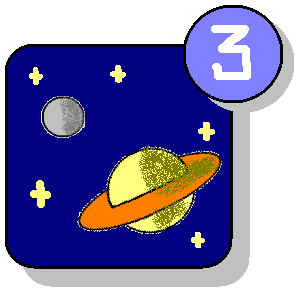
\includegraphics[scale=0.333]{cycle3-logo-espace.png}
% 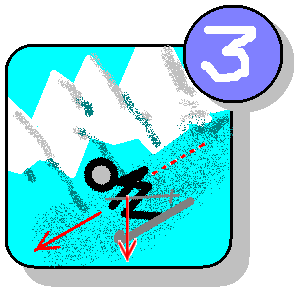
\includegraphics[scale=0.333]{cycle3-logo-mvts.png}
% 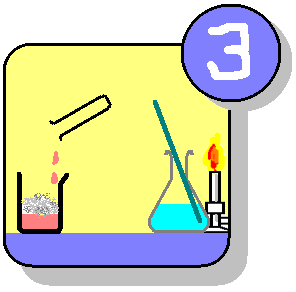
\includegraphics[scale=0.333]{cycle3-logo-transfo-matiere.png}
% 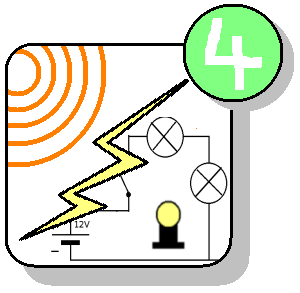
\includegraphics[scale=0.333]{cycle4-logo-elec-ondes-nrj.png}
% 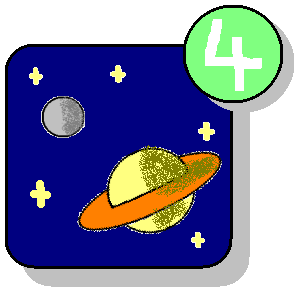
\includegraphics[scale=0.333]{cycle4-logo-espace.png}
% 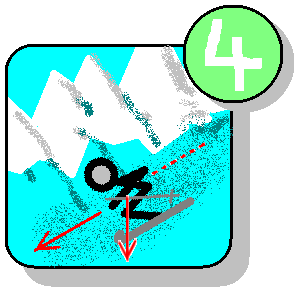
\includegraphics[scale=0.333]{cycle4-logo-mvts.png}
% 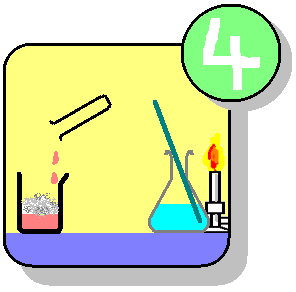
\includegraphics[scale=0.333]{cycle4-logo-transfo-matiere.png}

\ifthenelse{\boolean{isEvaluation}}{% True
\begin{flushleft}
\begin{tabular}{| m{0.15\linewidth} | m{0.8\linewidth} ||}
	\hline
	NOTE : & APPRÉCIATION : \cr
	$ ~~ $ & $ ~~ $ \cr
	$ ~~ $ & $ ~~ $ \cr
	$ ~~ $ & $ ~~ $ \cr
	$ ~~ $ & $ ~~ $ \cr
	$ ~~ $ & $ ~~ $ \cr
	\hline\hline
\end{tabular}
\end{flushleft}
}{% False
	\relax
} % end evaluation

\begin{flushleft}
\begin{tabular}{| m{0.03\linewidth} | m{0.75\linewidth} || m{0.015\linewidth} | m{0.015\linewidth} | m{0.015\linewidth} | m{0.015\linewidth} || }
\hline
\multirow{2}{*}{Ref} & \multirow{2}{*}{i~n~t~i~t~u~l~é~~~ d~e~~~ l~a~~~ c~o~m~p~é~t~e~n~c~e (cycle4) } & \multicolumn{4}{c ||}{É~t~a~t} \cr
	\cline{3-6}
	& & I & F & S & T \cr \hline
% A & Pratiquer des démarches scientifiques \cr \hline
%	A1 & \footnotesize{Identifier des questions de nature scientifique.} & & & & \cr \hline
%	A2 & \footnotesize{Proposer une ou des hypothèses pour répondre à une question scientifique. \newline Concevoir une expérience pour la ou les tester.} & & & & \cr \hline
	A3 & \footnotesize{Mesurer des grandeurs physiques de manière directe ou indirecte.} & & & & \cr \hline
	A4 & \footnotesize{Interpréter des résultats expérimentaux, en tirer des conclusions et les communiquer en argumentant.} & & & & \cr \hline
%	A5 & \footnotesize{Développer des modèles simples pour expliquer des faits d'observations et mettre en \oe{}uvre des démarches propres aux sciences.} & & & & \cr \hline
% B & Concevoir, créer, réaliser \cr \hline
	%B1 & \footnotesize{Concevoir et réaliser un dispositif de mesure ou d'observation.} & & & & \cr \hline
% C & S'approprier des outils et des méthodes \cr \hline
%	C1 & \footnotesize{Effectuer des recherches bibliographiques.} & & & & \cr \hline
% C2 & \footnotesize{Utiliser des outils numériques pour mutualiser des informations sur un sujet scientifique.} & & & & \cr \hline
%	C3 & \footnotesize{Planifier une tâche expérimentale, organiser son espace de travail, garder des traces des étapes suivies et des résultats obtenus.} & & & & \cr \hline
% D & Pratiquer des langages \cr \hline
%	D1 & \footnotesize{Lire et comprendre des documents scientifiques.} & & & & \cr \hline
%	D2 & \footnotesize{Utiliser la langue française en cultivant précision, richesse de vocabulaire et syntaxe pour rendre compte des observations, expériences, hypothèses et conclusions.} & & & & \cr \hline
%	D3 & \footnotesize{S'exprimer à l'oral lors d'un débat scientifique.} & & & & \cr \hline
%	D4 & \footnotesize{Passer d'une forme de langage scientifique à une autre.} & & & & \cr \hline
% E & Mobiliser des outils numériques \cr \hline
	E1 & \footnotesize{Utiliser des outils d'acquisition et de traitement de données, de simulations et de modèles numériques.} & & & & \cr \hline
%	E2 & \scriptsize{Produire des documents scientifiques grâce à des outils numériques, en utilisant l'argumentation et le vocabulaire spécifique à la physique et à la chimie.} & & & & \cr \hline
% F & Adopter un comportement éthique et responsable \cr \hline
%	F1 & \scriptsize{Expliquer les fondements des règles de sécurité en chimie, électricité et acoustique. Réinvestir ces connaissances ainsi que celles sur les ressources et sur l'énergie, pour agir de façon responsable.} & & & & \cr	\hline
%	F2 & \footnotesize{S'impliquer dans un projet ayant une dimension citoyenne.} & & & & \cr	\hline
% G & Se situer dans l'espace et dans le temps \cr \hline
%	G1 & \footnotesize{Expliquer, par l'histoire des sciences et des techniques, comment les sciences évoluent et influencent la société.} & & & & \cr	\hline
%	G2 & \footnotesize{Identifier les différentes échelles de structuration de l'Univers.} & & & & \cr \hline
	\hline
\end{tabular}
\end{flushleft}
% ============= DÉBUT DU DOCUMENT DE TRAVAIL ==================
\section*{Objectifs}
\begin{enumerate}
	\item Établir le lien qualitatif entre hauteur et fréquence d'un son et son tracé sur oscillogramme. 
	\item Établir le lien qualitatif entre intensité d'un son et le tracé sur un oscillogramme.
\end{enumerate}

\section*{Matériel et captures d'écran commentées.}
\subsection*{Le matériel}
Chaque groupe dispose :
\begin{itemize}
	\item de deux tablettes ou smartphones mis à disposition.
	\item des logiciels \texttt{signal generator} et \texttt{Tuner} (visualisateur)
\end{itemize}

\subsection*{Signal Generator}
Afin de vous familiariser avec le logiciel, voici une description visuelle de l'application \og~signal generator~\fg{}.
\begin{figure}
	\centering
	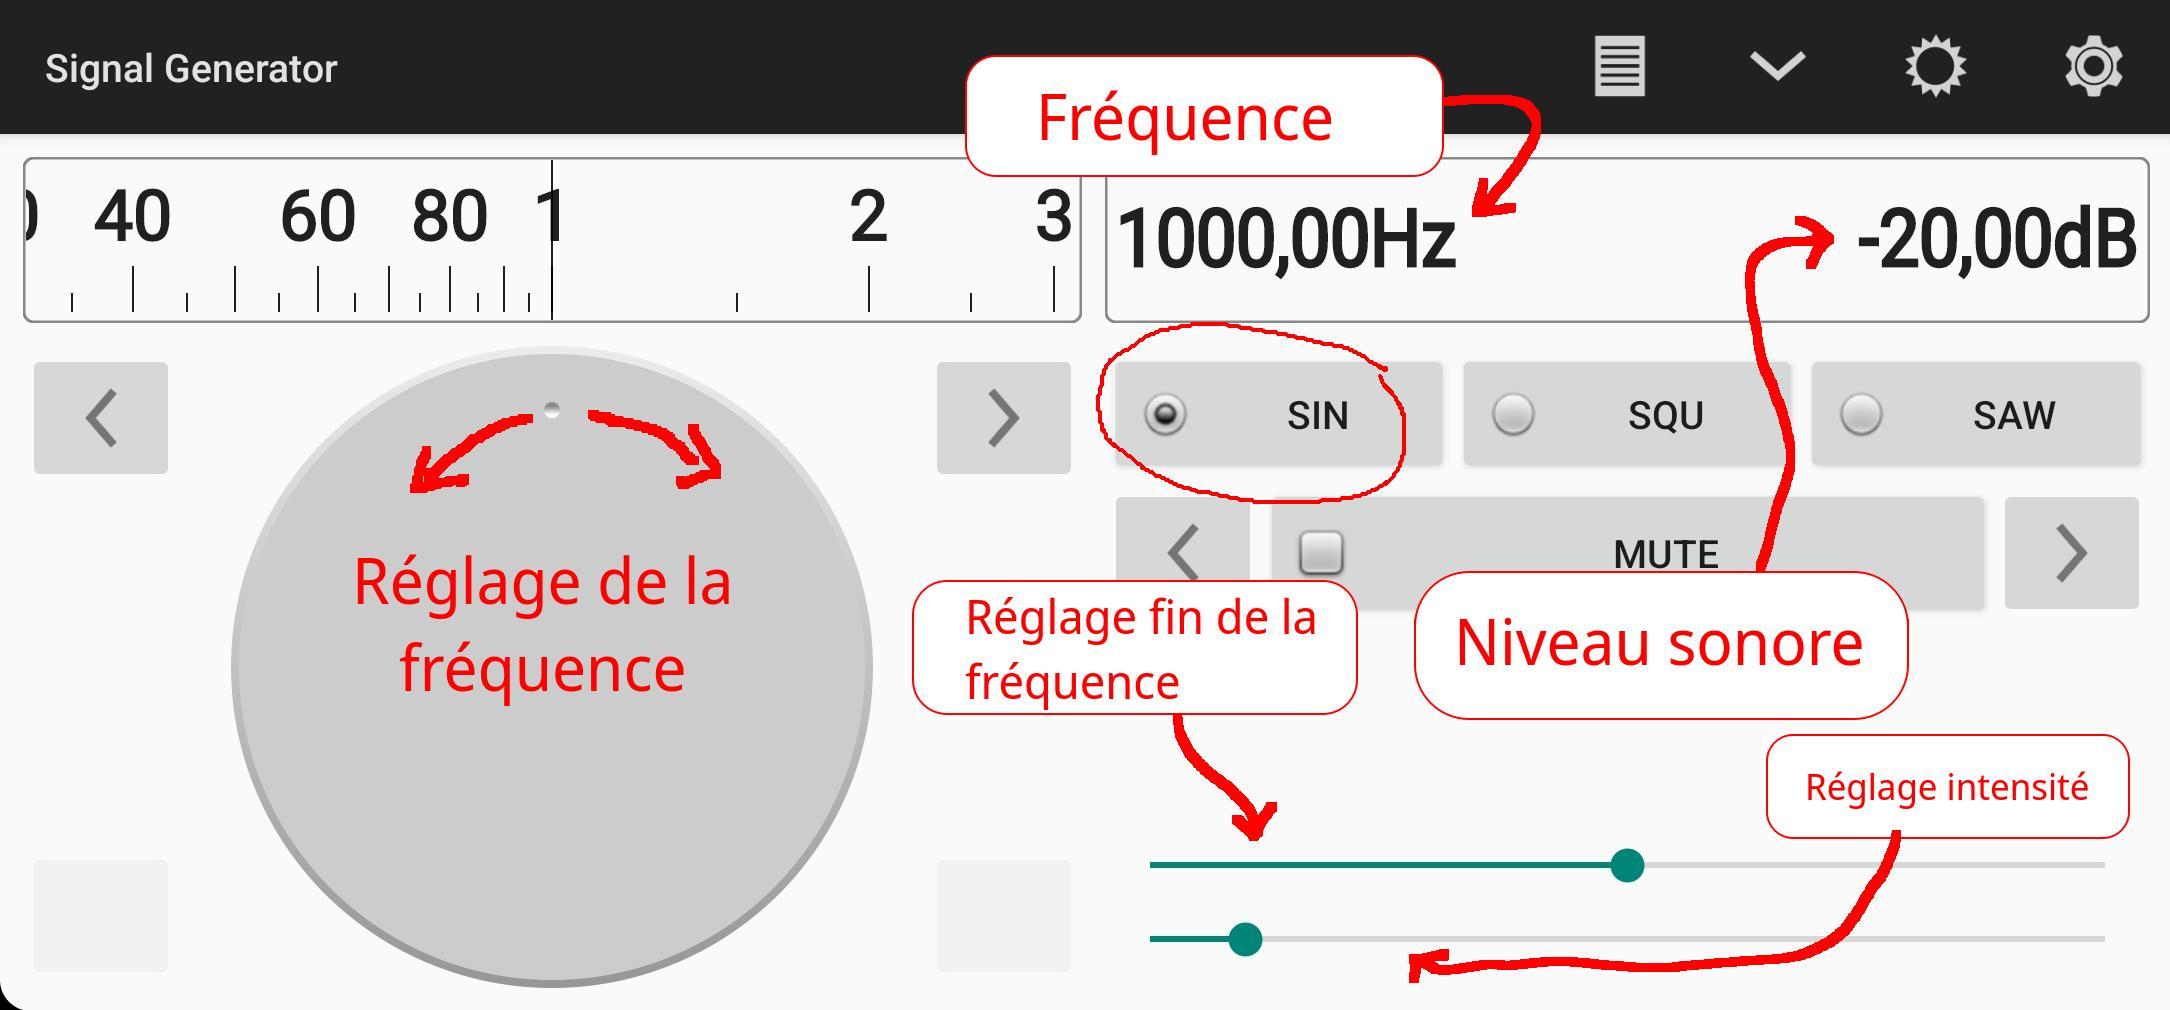
\includegraphics{signal-generator-1kHz.jpg} ;
\end{figure}

\subsection*{Tuner}
Afin de vous familiariser avec le logiciel, voici une description visuelle de l'application \og~Tuner~\fg{}.\begin{figure}
	\centering
	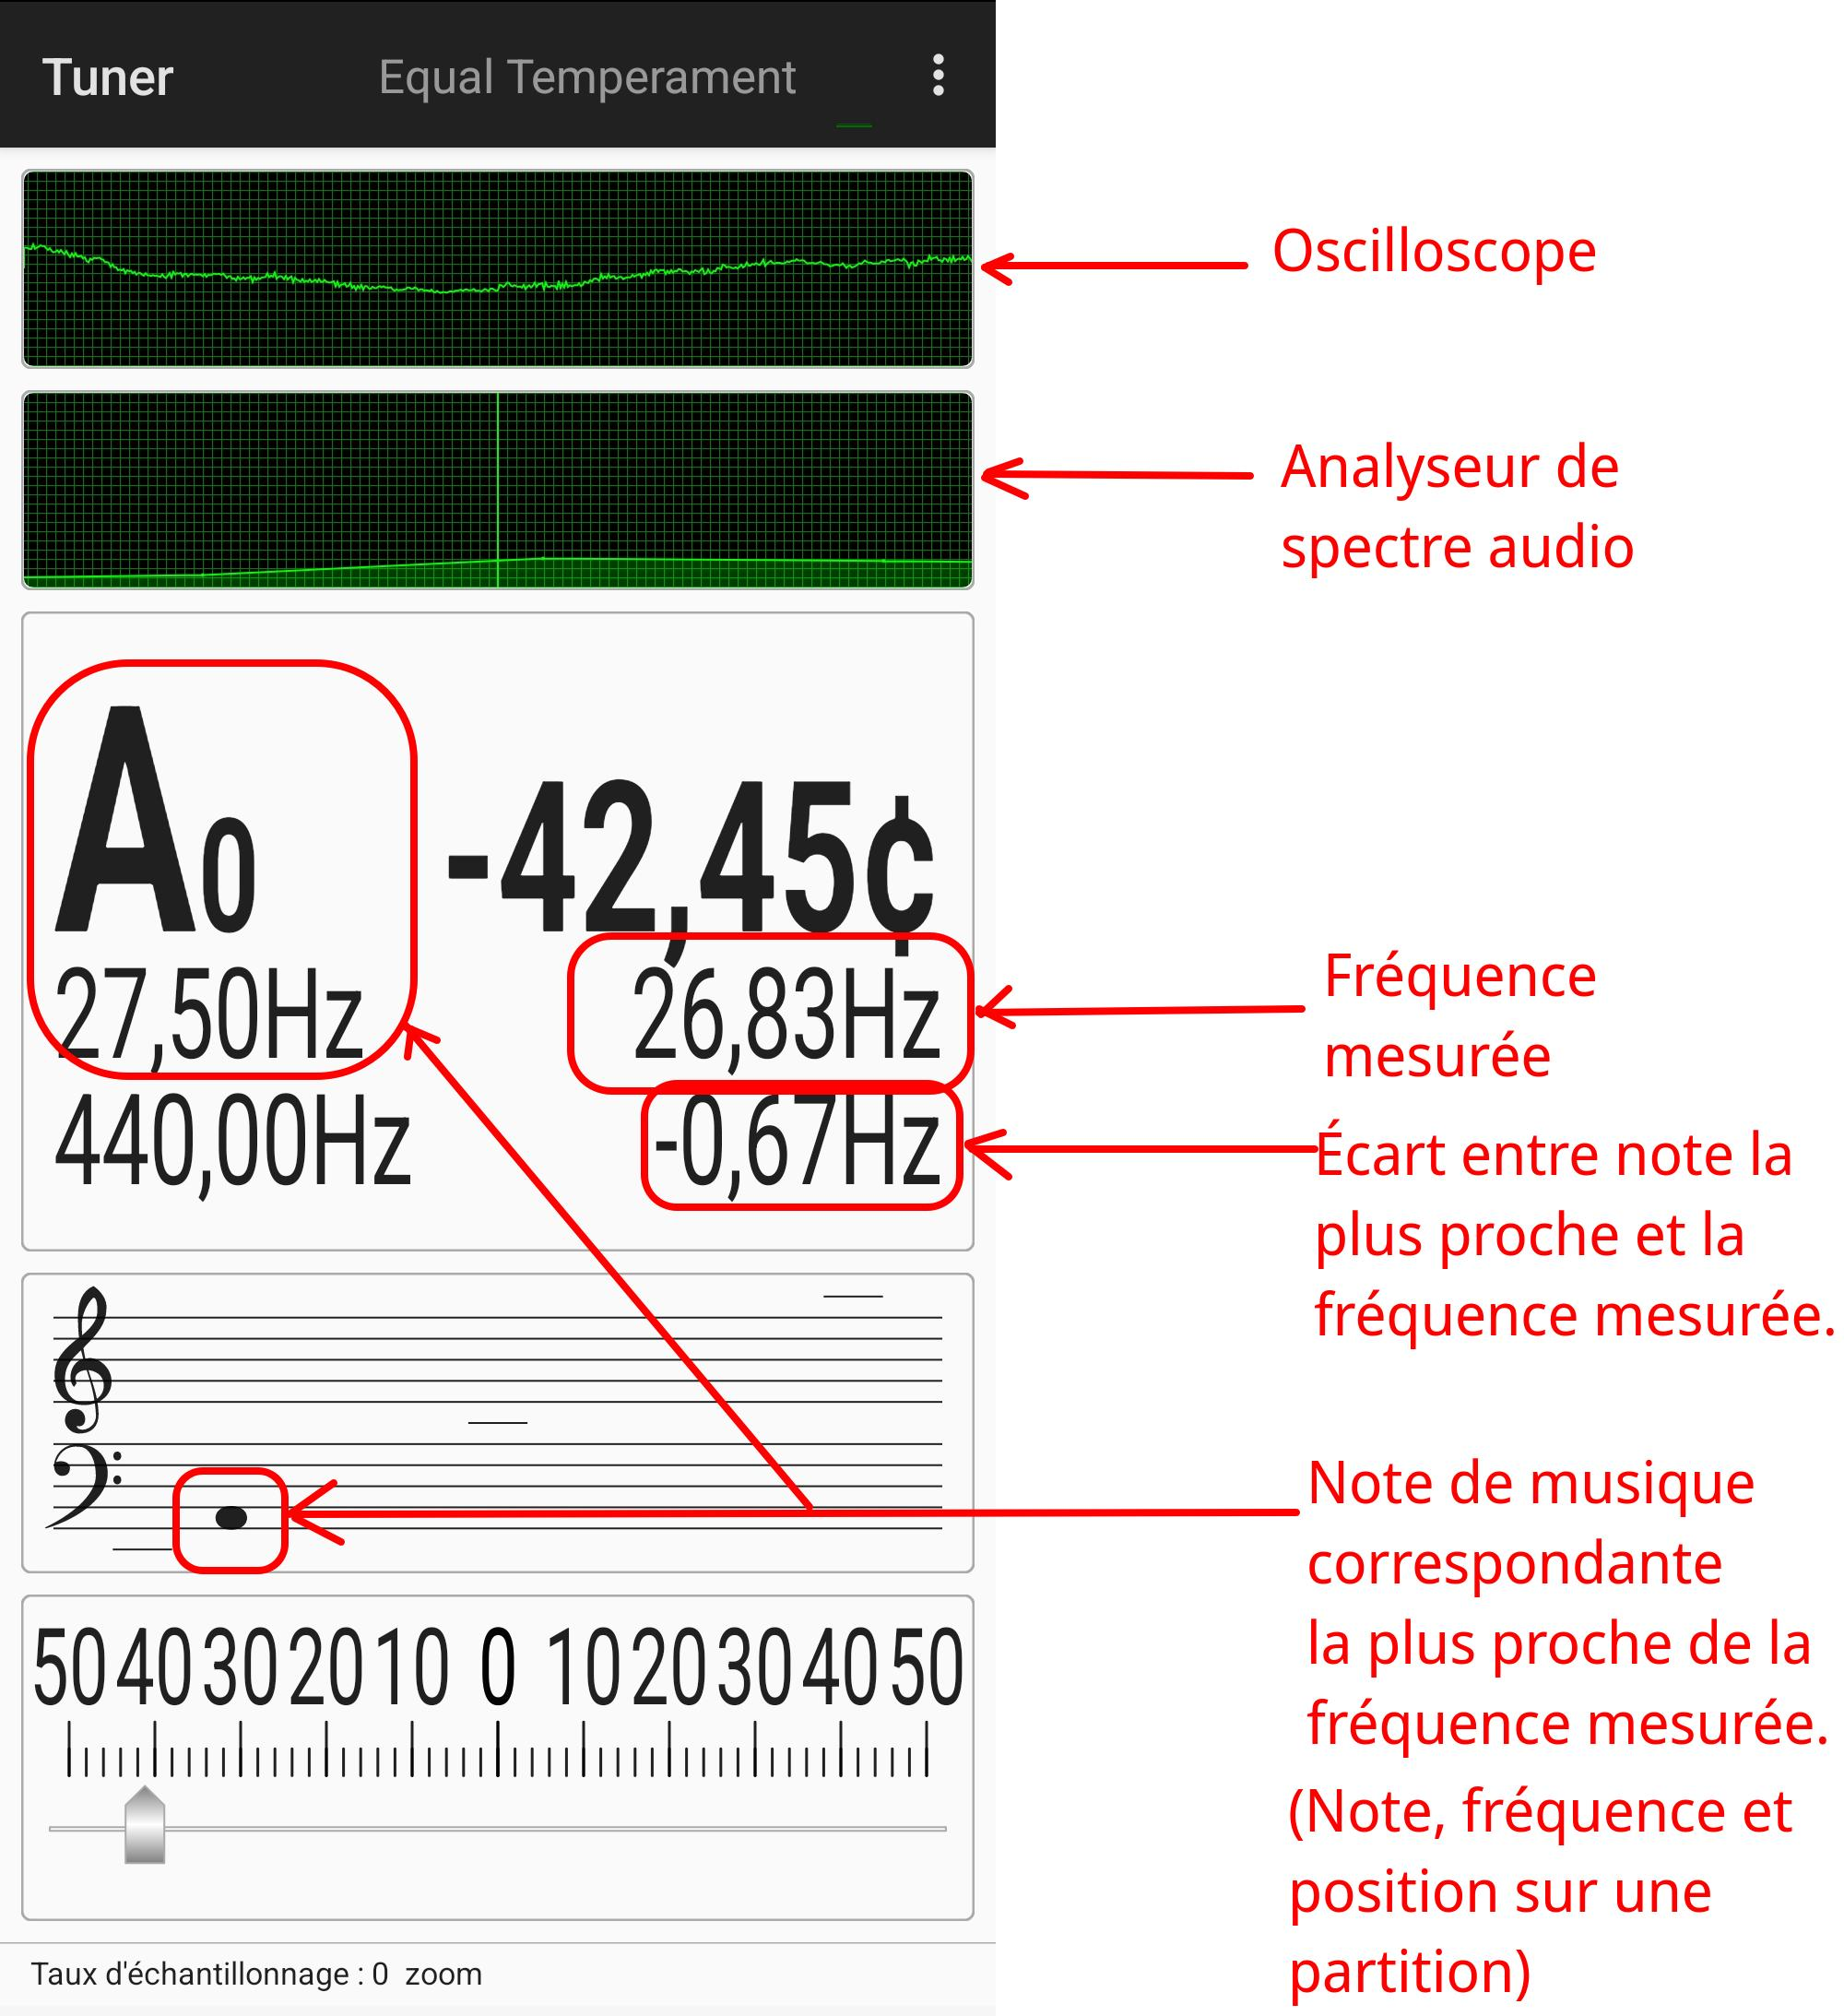
\includegraphics{Tuner.jpg}
\end{figure}

\section{Manipulations}
\begin{multicols}{2}
\paragraph{Description.}
Placez le haut-parleur de la tablette A exécutant l'application \emph{signal generator\/} contre le microphone de la tablette B exécutant l'application \emph{tuner\/}. 
Réglez le volume (avec les boutons) de la tablette 
Suivez ensuite les consignes.
\columnbreak

\begin{figure}
	\centering
	\begin{tikzpicture}
		\draw[rounded corners, fill=white!80!blue, line width=2pt] (5,0) rectangle ++(-3,2) node[below right] {{\tiny H.P.}} ;
		\draw[rounded corners, fill=white!80!blue, line width=2pt] (2.5,2.15) node[above left] {{\tiny micro}} rectangle ++(-2,3) ;
		\node (A) at (3.5,1) {tablette A} ;
		\node (B) at (1.5,3.65) {tablette B} ;
	\end{tikzpicture}
\end{figure}
\end{multicols}

\paragraph{1\iere{} manipulation.}
Réglez la tablette A de la façon suivante~:
\begin{itemize}
	\item son à moitié du maximum (boutons physiques)
	\item Fréquence F~=~440,00~Hz
	\item forme du signal sur $\boxed{\circ ~ \rm sin}$
	\item intensité sonore réglée à -20~dB.
\end{itemize}
Changez ensuite la fréquence dans l'application \emph{signal generator\/} et observez les changements dans l'application \emph{Tuner\/}. 
Complétez le tableau qui suit avec vos mesures (au moins 5).
\begin{table}
	\centering
	\caption{Mesures de la première manipulation.}
	\renewcommand*{\arraystretch}{1.45}
	\rowcolors{1}{white!95!blue}{white}
	\begin{tabular}{| m{0.11\linewidth} | m{0.18\linewidth} | m{0.64\linewidth} |}
		\hline
		Fréq. (Hz) & Hauteur ($\pm$ aigu) & Description du tracé (oscillogramme) \cr
		\hline
		& & \cr
		\hline
		& & \cr
		\hline
		& & \cr
		\hline
		& & \cr
		\hline
		& & \cr
		\hline
	\end{tabular}
\end{table}

\paragraph{2\ieme{} manipulation.} 
Réglez la tablette A de la façon suivante~:
\begin{itemize}
	\item volume à la moitié du maximum (boutons physiques)
	\item Fréquence F~=~440,00~Hz
	\item forme du signal sur $\boxed{\circ ~ \rm sin}$
	\item intensité sonore réglée à -20~dB.
\end{itemize}
Changez l'intensité sonore à l'aide du curseur. Notez ce qui se passe dans l'oscillogramme dans les pointillés qui suivent.

\paragraph*{Notes.}
. \ \ . \ \ . \ \ . \ \ . \ \ . \ \ . \ \ . \ \ . \ \ . \ \ . \ \ . \ \ . \ \ . \ \ . \ \ . \ \ . \ \ . \ \ . \ \ . \ \ . \ \ . \ \ . \ \ . \ \ . \ \ . \ \ . \ \ . \ \ . \ \ . \ \ . \ \ . \ \ . \ \ . \ \ . \ \ . \ \ . \ \ . \ \ . \ \ . \ \ . \ \ . \ \ . \ \ . \ \ . \ \ . \ \ . \ \ . \ \ . \ \ . \ \ . \ \ . \ \ . \ \ . \ \ . \ \ . \ \ . \ \ . \ \ . \ \ . \ \ . \ \ . \ \ . \ \ . \ \ . \ \ . \ \ . \ \ . \ \ . \ \ . \ \ . \ \ . \ \ . \ \ . \ \ . \ \ . \ \ . \ \ . \ \ . \ \ . \ \ . \ \ . \ \ . \ \ . \ \ . \ \ . \ \ . \ \ . \ \ . \ \ . \ \ . \ \ . \ \ . \ \ . \ \ . \ \ . \ \ . \ \ . \ \ . \ \ . \ \ . \ \ . \ \ . \ \ . \ \ . \ \ . \ \ . \ \ . \ \ . \ \ . \ \ .

\paragraph{3\ieme{} manipulation.} 
Réglez la tablette A de la façon suivante~:
\begin{itemize}
	\item volume à la moitié du maximum (boutons physiques)
	\item Fréquence F~=~440,00~Hz
	\item forme du signal sur $\boxed{\circ ~ \rm sin}$
	\item intensité sonore réglée à -20~dB.
\end{itemize}
Modifiez la distance entre le micro de la tablette B et le haut-parleur de la tablette A. 
Notez ce qui se passe dans l'oscillogramme dans les pointillés qui suivent. 

\paragraph*{Notes.}
. \ \ . \ \ . \ \ . \ \ . \ \ . \ \ . \ \ . \ \ . \ \ . \ \ . \ \ . \ \ . \ \ . \ \ . \ \ . \ \ . \ \ . \ \ . \ \ . \ \ . \ \ . \ \ . \ \ . \ \ . \ \ . \ \ . \ \ . \ \ . \ \ . \ \ . \ \ . \ \ . \ \ . \ \ . \ \ . \ \ . \ \ . \ \ . \ \ . \ \ . \ \ . \ \ . \ \ . \ \ . \ \ . \ \ . \ \ . \ \ . \ \ . \ \ . \ \ . \ \ . \ \ . \ \ . \ \ . \ \ . \ \ . \ \ . \ \ . \ \ . \ \ . \ \ . \ \ . \ \ . \ \ . \ \ . \ \ . \ \ . \ \ . \ \ . \ \ . \ \ . \ \ . \ \ . \ \ . \ \ . \ \ . \ \ . \ \ . \ \ . \ \ . \ \ . \ \ . \ \ . \ \ . \ \ . \ \ . \ \ . \ \ . \ \ . \ \ . \ \ . \ \ . \ \ . \ \ . \ \ . \ \ . \ \ . \ \ . \ \ . \ \ . \ \ . \ \ . \ \ . \ \ . \ \ . \ \ . \ \ . \ \ . \ \ .

\section{Conclusion}
En utilisant les résultats des trois manipulations, que pouvez-vous dire sur le lien entre hauteur d'un son, sa fréquence et son tracé sur un oscillogramme~? Même chose avec l'intensité sonore du son et son tracé sur l'oscillogramme.
\begin{bclogo}[couleur=yellow!5, arrondi=0.1, logo=\bccrayon, nobreak=true]{}

\ifthenelse{\boolean{isCorrection}}{% true
{\large Plus un son est aigu plus sa fréquence et élevée et plus les vaguelettes sur un oscillogramme sont serrées, à \emph{contrario\/} si le son est grave, sa fréquence est basse et les vaguelettes élargies. \newline
Pour l'intensité sonore, plus le son est fort, plus les maxima et minima de la courbe sont écartés.}
}{%false
\noindent . \ \ . \ \ . \ \ . \ \ . \ \ . \ \ . \ \ . \ \ . \ \ . \ \ . \ \ . \ \ . \ \ . \ \ . \ \ . \ \ . \ \ . \ \ . \ \ . \ \ . \ \ . \ \ . \ \ . \ \ . \ \ . \ \ . \ \ . \ \ . \ \ . \ \ . \ \ . \ \ . \ \ . \ \ . \ \ . \ \ . \ \ . \ \ . \ \ . \ \ . \ \ . \ \ . \ \ . \ \ . \ \ . \ \ . \ \ . \ \ . \ \ . \ \ . \ \ . \ \ . \ \ . \ \ . \ \ . \ \ . \ \ . \ \ . \ \ . \ \ . \ \ . \ \ . \ \ . \ \ . \ \ . \ \ . \ \ . \ \ . \ \ . \ \ . \ \ . \ \ . \ \ . \ \ . \ \ . \ \ . \ \ . \ \ . \ \ . \ \ . \ \ . \ \ . \ \ . \ \ . \ \ . \ \ . \ \ . \ \ . \ \ . \ \ . \ \ . \ \ . \ \ . \ \ . \ \ . \ \ . \ \ . \ \ . \ \ . \ \ . \ \ . \ \ . \ \ . \ \ . \ \ . \ \ . \ \ . \ \ . \ \ . \ \ . \ \ . \ \ . \ \ . \ \ . \ \ . \ \ . \ \ . \ \ . \ \ . \ \ . \ \ . \ \ . \ \ . \ \ . \ \ . \ \ . \ \ . \ \ . \ \ . \ \ . \ \ . \ \ . \ \ . \ \ . \ \ . \ \ . \ \ . \ \ . \ \ . \ \ . \ \ . \ \ . \ \ . \ \ . \ \ . \ \ . \ \ . \ \ . \ \ . \ \ . \ \ . \ \ . \ \ . \ \ . \ \ . \ \ . \ \ . \ \ . \ \ . \ \ . \ \ . \ \ . \ \ . \ \ . \ \ . \ \ . \ \ . \ \ . \ \ . \ \ . \ \ . \ \ . \ \ . \ \ . \ \ . \ \ . \ \ . \ \ . \ \ . \ \ . \ \ . \ \ . \ \ . \ \ . \ \ . \ \ . \ \ . \ \ . \ \ . \ \ . \ \ . \ \ . \ \ . \ \ . \ \ . \ \ . \ \ . \ \ . \ \ . \ \ . \ \ . \ \ . \ \ . \ \ . \ \ . \ \ . \ \ . \ \ . \ \ . \ \ . \ \ . \ \ . \ \ . \ \ . \ \ . \ \ . \ \ . \ \ .
}
\end{bclogo}

\end{document}
%%%%%%%%%%%%%%%%%%%%%%%%%%%%%%%%%%%%%%%%%%%%%%%%%%%%%%%%%%%%%%%

% cadre pour le cours / à savoir par coeur.
\begin{bclogo}[couleur=pink!5, epOmbre=0.2cm, arrondi=0.1, logo=\bccoeur, nobreak=true]{}

\end{bclogo}

% cadre pour un document à analyser (informatif)
\begin{bclogo}[couleur=blue!5, epOmbre=0.2cm, arrondi=0.1, logo=\bcinfo, nobreak=true]{}

\end{bclogo}

% cadre pour le travail :
\begin{bclogo}[couleur=yellow!5, arrondi=0.1, logo=\bccrayon, nobreak=true]{}

\end{bclogo}
